
\documentclass[5p,sort&compress]{elsarticle}		

\makeatletter
\def\ps@pprintTitle{%
 \let\@oddhead\@empty
 \let\@evenhead\@empty
 \def\@oddfoot{\footnotesize\itshape
    
    
       \hfill\today}%
 \let\@evenfoot\@oddfoot}
\makeatother

\usepackage{lmodern}
\usepackage{amsmath}
\usepackage{amssymb}
\usepackage{bm}
\usepackage{siunitx}
\usepackage{graphicx} 

\renewcommand{\topfraction}{.85}
\renewcommand{\bottomfraction}{.7}
\renewcommand{\textfraction}{.15}
\renewcommand{\floatpagefraction}{.66}
\setcounter{topnumber}{3}
\setcounter{bottomnumber}{2}
\setcounter{totalnumber}{10}

\usepackage{flafter}
\usepackage{booktabs}
\usepackage{multirow}
\usepackage[font=small,labelfont=bf]{caption}
\usepackage[colorlinks=true,allcolors=blue]{hyperref}
\urlstyle{same}

\begin{document}
\begin{frontmatter}

\title{Surface Emissivity and Vericifation of Stefan-Boltzmann Law}

\author[physics]{M. D.~Tat}
\author[physics]{W.~Dugan}

\address[Physics]{Institution of Physics, Norwegian University of Science and Technology, 7491 Trondheim.}

\begin{abstract}
The intensity of thermal radiation depends on a body's temperature and the emissivity of the body's surface. Here, Leslie's cube and a lamp with tungsten fillament were used to study the emissivity of different surfaces and temperatures of an idealised black body. Our standard mean error (SME) of relative emissivity across the surfaces were, at most, $0.008$, and temperature uncertainty of the lamp was $1.46\times10^{11}$ K$^4$. In conclusion, the emissivity of a body is independent of temperature, but depends on the surface material, and the intensity of thermal radiation for a black body is proportional the fourth power of temperature.

% The second experiment regarding the lamp with Tungsten fillament showed that the thermal radiation emitted from a body is dependent on the temperature of the body and follows the relation given in \eqref{eq:stefanboltzmann}.

\end{abstract}
\end{frontmatter}

%------------INTRO--------------------
\section{Introduction}

Thermal radiation is a process in which a hot body emits energy in the form of electromagnetic radiation. It is characterised by the temperature of the body. We may categorize objects by their emissivity. That is, a black body is an object that absorbs all incident radiation, while a grey body absorbs some of the incident radiation, and reflects the remaining. A good absorber is also a good emitter of energy, according to Kirchhoff's law of thermal radiation~\cite{britannica}.

This lab report concerns both an idealised black body and a number of grey bodies. Two experiments were carried out to study the relationship between the emitted thermal radiation by hot bodies and their temperatures. 

The first experiment concerns the emissivity of different surfaces. We will study these surfaces in relation to Kirchhoff's law of thermal radiation and the temperature of the body. To do this, a Leslie's Cube is heated and the emitted thermal radiation is measured using a sensor. Leslie's Cube is a cube with four different surfaces: matte white, matte black, polished aluminium, and dull aluminium. It is heated from the inside with a light bulb. The sensor used is a PASCO TD-8553 Radiation Sensor which uses the thermoelectric effect to measure the temperature of the body. 

The second experiment investigates Stefan-Boltzmann's law using a lamp with tungsten filament as an idealised black body. Here, we measure the radiation intensity at different temperatures. 

The motivation for this report is that it serves as an exercise for us students to develop the necessary skills required to do academic research. Furthermore, it serves as a demonstration of thermodynamic laws and thus enhances our understanding of them.

%------------THEORY--------------------
\section{Theory}
Stefan-Boltzmann Law states the following:
\begin{equation}
    j = \varepsilon\sigma T^4
    \label{eq:stefanboltzmann}
\end{equation}
where $j$ is the intensity of thermal radiation,  $\varepsilon$ is the emissivity, $\sigma$ is the Stefan-Boltzmann constant, and $T$ is the absolute temperature. The thermal emissivity is a ratio between the intensity of heat radiation and that of a black body. Hence, for black bodies, this value is given as $\varepsilon =1$, while for grey bodies we have $0< \varepsilon <1$. In the first experiment, we investigate the different $\varepsilon$ values for various surfaces. 

In the first experiment, we measure the relative radiation intensity and calculate the emissivity of all surfaces and temperatures. Then, we can see how the emissivity depends on the different parameters.

In the second experiment, we want to verify equation \eqref{eq:stefanboltzmann}. This was done by looking at the relationship between the relative intensity and temperature. To find the temperature, we calculate the the resistance in the lamp by measuring the potential and current over it. We could then use the ratio $R/R_0$ and Table 2 in~\cite{pasco} to determine the corresponding temperature for each resistance value. $R_0$ is the internal resistance of the lamp which was measured precisely using a wheatstone bridge.

\subsection{Wheatstone bridge}
\begin{figure}[t]
    \centering
    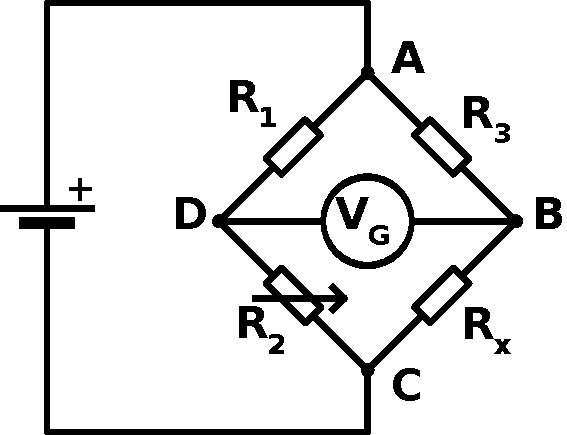
\includegraphics[width=0.25\textwidth]{../wheatstone_bridge.pdf}
    \caption{Circuit diagram of a Wheatstone bridge. From~\cite{wheatstone_fig}.}
    \label{fig:wheatstone}
\end{figure}
When the current $V_G$ is zero, the equation 
\begin{align}
    R_x = \frac{R_2 \cdot R_3}{R_1}
\end{align}
holds, where $R_1,\ R_2,\ R_3$ are known to high precision. To find the resistance of the lamp, one can measure the resistance of the lamp and the wires, and then subtract the measured resistance in only the wires.

%------------ERROR PROP--------------------
\subsection{Error Analysis}
The standard error will be used to determine the precision of the results from Leslie's cube experiment and is calculated as follows
\begin{equation}
    \delta \bar \varepsilon 
    = \frac{\sigma_{\varepsilon}}{\sqrt{N}} 
    = \frac{\sum^N_i\sqrt{  \frac{(\varepsilon_i-\bar\varepsilon)^2}{N-1}}}{\sqrt N} \text{,}
\end{equation}
where $\varepsilon$ is the relative emissivity between a surface and the surface with largest emissivity, $\bar \varepsilon$ is the mean relative emissivity for said surface, and $N$ is the number of relative emissivity that was measured.  

For the tungsten lamp, the uncertainty of the resistance, $\delta R$, is calculated using $\delta V = 0.01$ V and $\delta I = 1$ mA. With $\delta R_0 = 1$ m$\Omega$, we get $\langle\delta R / R_0 \rangle = 0.26\% + 0.36\% = 0.62\%$. This is very small. Table 2 in~\cite{pasco} has incremental temperatures of 100 K, so we estimated $\delta T = 50$ K rather than using $\delta R / R_0$ to calculate the error in temperature.

\section{Method}
\subsection{Leslie's Cube}
\begin{figure}[h]
    \centering
    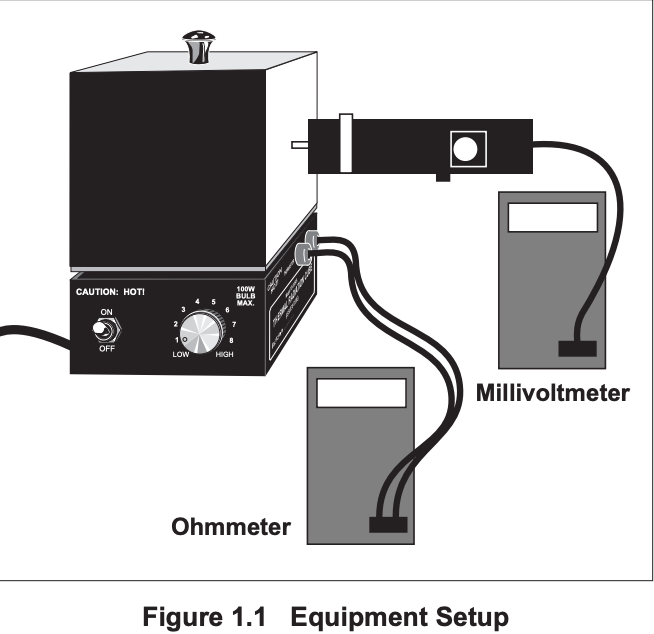
\includegraphics[width=0.35\textwidth]{../setup_1.png}
    \caption{Drawing of the first experiment. From~\cite{pasco}.}
    \label{fig:setup_1}
\end{figure}

The setup is as illustrated in \autoref{fig:setup_1}. Leslie's cube was connected to a digital multimeter set to k$\Omega$. The sensor was connected to a digital multimeter set to mV. The cube was then preheated at the maximum power setting untill it reached thermal equilibrium, meaning that the ohmmeter was fluctuating about a set value. Once the cube reached thermal equilibrium, the power setting was turned down. Then, data was gathered by placing the sensor in contact with the surface and note down the voltmeter and ohmmeter readings. 

This was repeated for all four surfaces. The power setting was then increased, and the data gathering process was repeated once the cube reached thermal equilibrium. The whole experiment was repeated for 4 different power settings. 

\subsection{Stefan-Boltzmann Lamp}
\begin{figure}[h]
    \centering
    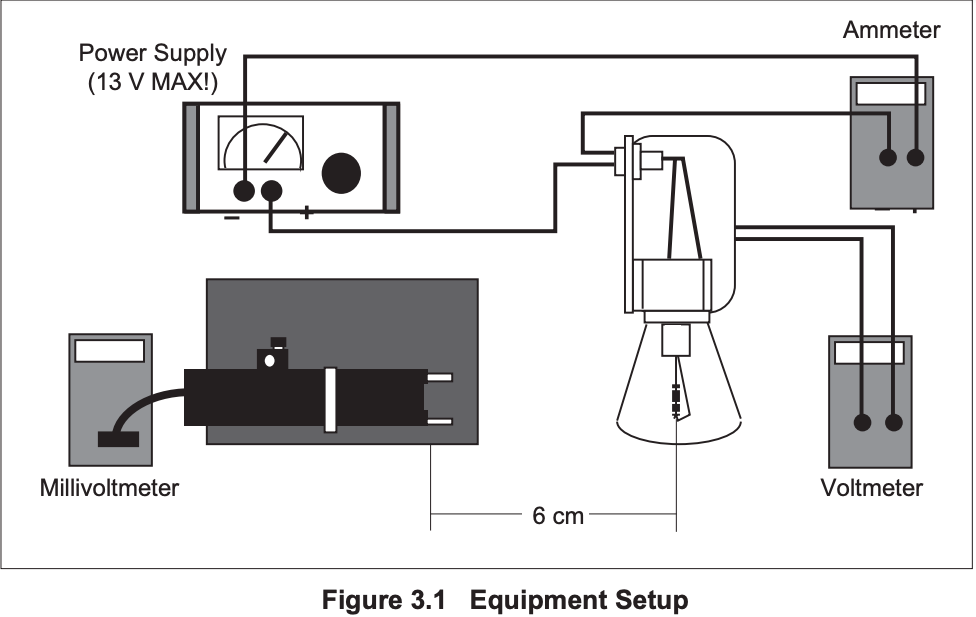
\includegraphics[width=0.45\textwidth]{../setup_2.png}
    \caption{Drawing of the second experiment. From~\cite{pasco}.}
    \label{fig:setup_2}
\end{figure}

Before the setup, a wheatstone bridge was used to measure the resistance over the lamp.

The setup is seen in \autoref{fig:setup_2}. The lamp was connected in series to a power supply
and ammeter, and in parallel to a voltmeter, while the sensor remained connected to the voltmeter. After that, a heat shield was placed between the lamp and the sensor. The shield purpose is to prevent heating of the sensor. To gather data, the voltage was first set to 1 V, and the current on the power supply adjusted accordingly to get 1 V throught the lamp as well. The shield was removed and the radiation, potential, and current were noted down. The shield was placed back in between the sensor and lamp. The voltage increased by 1 V per measurement. This was repeated 12 times for a voltage and current in the range of 1 V to 12 V and approximately 1 A to 3 A, respectively. 

%-------------RESULTS--------------
\section{Results}
\subsection{Leslie's Cube}
\begin{table}[ht] 
\centering
    \begin{tabular}{||c|c||}
    	\hline
        \text{Surface} & $ \bar \varepsilon$ [-]\\
        \hline
        \text{Black} & $1.000$\\
        \text{White} & $0.966  \pm 0.004$\\
        \text{Dull Al} & $0.078 \pm 0.002$ \\
        \text{Polished Al} & $0.363 \pm 0.008$ \\
        \hline
    \end{tabular}
    \caption{Mean relative thermal emissivity for different surfaces with the corresponding standard error of the mean (SEM). $\bar \varepsilon = \bar \varepsilon_{\text{Surface}}/\bar \varepsilon_{\text{Black}}$}
    \label{cube}
\end{table}

The results of the first experiment is presented in \autoref{cube}. Here, $\bar\varepsilon_{\text{Surface}}$ is the average emissivity of the surface divided by the average emissivity of the black surface. 

The emissivity in an increasing order is as follows: black, white, dull aluminium, and polished aluminium. From~\autoref{cube} we see that the emissivity for the matte surfaces are close in magnitude, with $\bar \varepsilon_{\text{white}}= 0.966 \bar \varepsilon_{\text{black}}$, while the emissivity of for the aluminium surfaces are less than $40\%$ of the matte black emissivity, or $\bar \varepsilon_{\text{black}}> 0.4 \bar \varepsilon_{\text{Al}}$. 

\subsection{Stefan-Boltzmann Lamp}
\begin{figure}[h]
    \centering
    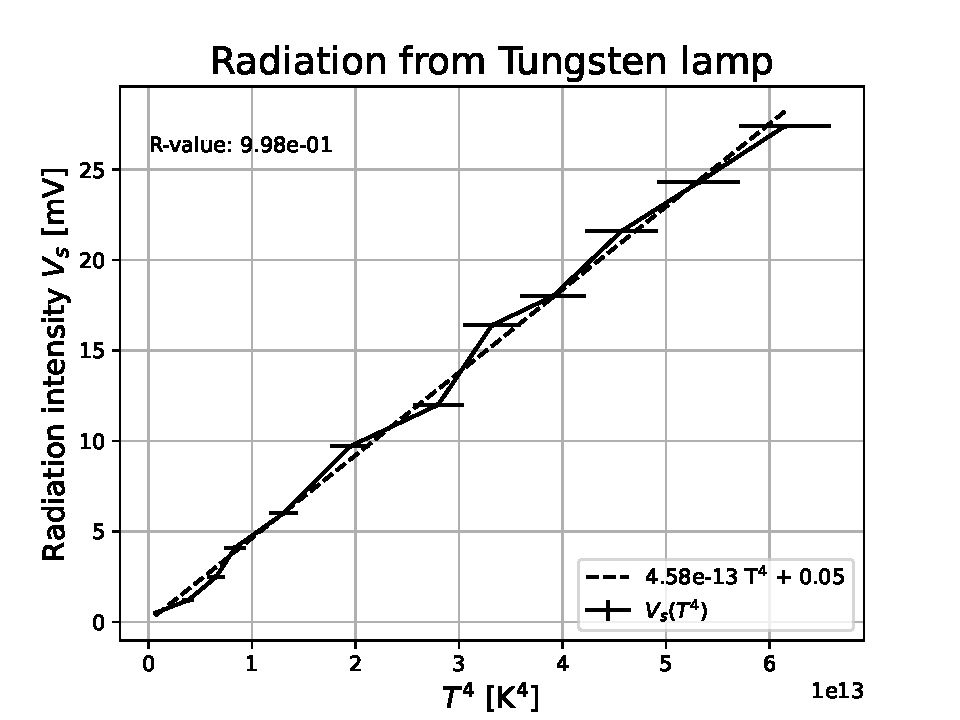
\includegraphics[width=0.5\textwidth]{../lamp.pdf}
    \caption{Plot of radiation intensity as a function of temperature together with a linear regression. Error bars omitted on y axis as they were not visible.}
    \label{fig:lamp}
\end{figure}

The internal resistance $R_0$ over the lamp was found to be ($0.278 \pm 0.001$) $\Omega$ using the Wheatstone bridge. The temperature was found as follows:
\begin{align*}
    R = V/I = 1.02 \text{ V} / 0.928 \text{ A} = 1.10 \\
    R / R_0 = 1.10 \ \Omega / 0.278 \  \Omega = 3.95 \\
    \rightarrow T = 900 \text{ K},\ T^4 = 6.56\cdot10^{11} \text{ K}^4 \\
    \delta T^4 = \sqrt{(4 \cdot 900^3 \cdot 50)^2} = 1.46\cdot 10^{11} \text{ K}^4
\end{align*}
This was done for all 12 data points in Python 3. The result is presented graphically in \autoref{fig:lamp}.

%-------------DISCUSSION--------------
\section{Discussion}
\subsection{Leslie's Cube}
From \autoref{cube} we see that the standard error of the mean (SEM) is small in comparison to the mean relative emissivity, $\bar\varepsilon$. This implies that the emissivity of a given surface is independent on the bodys temperature. The results also show that a matte surface have a higher emissivity compared to a more reflective one, such as polished aluminium.

% During the experiment, the thermistor was observed to fluctuated about $11 \text{ k}\Omega$ when the cube was in thermal equilibrium on the maximum power setting. The instructions stated that the resistance is supposed to fluctuate about $40\text{ k}\Omega$. We believe this has little to no effect on our results, as we are comparing trends.

\subsection{Stefan-Boltzmann Lamp}
In \autoref{fig:lamp} we see that the radiation intensity increases with temperature. Even though we would expect a linear graph from~\eqref{eq:stefanboltzmann}, this is not the case. Nevertheless, if we consider the error in temperature, we see that the linear regression passes through our uncertainty range. This is further confirmed by the $R^2$-value that is almost equal to 1, which is a measure on how close a regression is, where $R^2=1$ is a perfect correlation.

The regression line does not pass through $(0,0)$. We believe that the constant $+0.05$ comes from background thermal radiation, such as from the lights in the lab.

The larges deviations from the regression line is in the range $3\cdot10^{13}$ K$^4$. For these two measurements, we forgot to place the heat shield in between the lamp and the sensor. This shows how sensitive the sensor is to temperature changes.

The distance between the center was also a bit further than 6 cm, which is the distance stated in~\cite{pasco}. Regardless, the distance was kept constant and is assumed to have little effect on our results.

The uncertainty $\delta T^4$ is very high. This could ealisy have been significantly lower if we did a (linear) regression of Table 1 in~\cite{pasco}. By doing this, we could have calculated the error $\delta T^4$ from $\delta T_{R/R_0}$ instead of (over)estimating it to be 50 K.

%-------------CONCLUSION--------------
\section{Conclusion}
The first experiment regarding a Leslie's cube showed that the emissivity of a body is independent of its temperature, but dependent on the surface finish. The matte surfaces presented an emissivity of approximately 40\% more than the aluminium surfaces. 

The second experiment regarding the lamp with Tungsten fillament showed that the thermal radiation emitted from a body is dependent on the temperature of the body and follows the relation given in~\eqref{eq:stefanboltzmann}. Thus, we conclude that Stefan-Boltzmann's law holds.

%-------------REFERENCES--------------
\begingroup
\begin{center}
    \rule{2cm}{.4pt}
\end{center}
\makeatletter
\bibliographystyle{IEEEtran}
\bibliography{references.bib}

\end{document}
